\documentclass{article}
\usepackage[margin=1 in]{geometry}
\usepackage{listings}[language = R]
\usepackage[utf8]{inputenc}
\usepackage{graphicx}
\usepackage{listings}
\usepackage{xcolor}

\definecolor{codegreen}{rgb}{0,0.6,0}
\definecolor{codegray}{rgb}{0.5,0.5,0.5}
\definecolor{codepurple}{rgb}{0.58,0,0.82}
\definecolor{backcolour}{rgb}{0.95,0.95,0.92}

\lstdefinestyle{mystyle}{
    backgroundcolor=\color{backcolour},   
    commentstyle=\color{codegreen},
    keywordstyle=\color{magenta},
    numberstyle=\tiny\color{codegray},
    stringstyle=\color{codepurple},
    basicstyle=\ttfamily\footnotesize,
    breakatwhitespace=false,         
    breaklines=true,                 
    captionpos=b,                    
    keepspaces=true,                 
    numbers=left,                    
    numbersep=5pt,                  
    showspaces=false,                
    showstringspaces=false,
    showtabs=false,                  
    tabsize=2
}
\lstset{style=mystyle}
\usepackage[utf8]{inputenc}
\usepackage{xcolor}
\title{\vspace{-4em}Algorithm for Limit Prediction}
\author{HUA TONG \quad YUKUN FANG\quad ZIJUN FENG}
\date{September 2020}

\begin{document}
\maketitle
\section{Introduction}
 Our algorithm is to \textbf{develop an algorithm that can predict when hard drives will rich is maximum capacity} so that engineers can plan ahead and make adjustments to the server storage.\newline
 Based on the linear regression model which Professor gave to us, we upgrade the function to deal with some \textbf{specific situations} and write codes concisely to make fast and accurate predictions.
\section{Analysis}
 The Algorithm has four sections:\\
 \textbf{First}, we use same code as professor gave to remove the NAs and characters. Also we need to detect whether the end of y\_t is 0 or not. If true, remove it.\\
 \textbf{Second} Not only do we need to find breakpoints in y\_t but also mark down its beginning and ending.\\
 \textbf{Because} the breakpoints are made by engineers to update or maintenance system  which is not useful for us, we need to deal with it to let our prediction more accurately.\\
 \textbf{Then} use the linear interpolation to remedy the breaking part. It will help us to use linear model.\\
 \textbf{At last}use the linear mode for prediction but we do not use the \emph{lm} function. On the contrary, we use the formula of the linear regression to make it faster.
\section{Regular Test}
\subsection{Robustness/Error Tolerance}
This part is quite easy for our project and we use the same codes as example.
\subsection{Accuracy}
Because we have made our prediction more earlier for protection, for this small sample data there exists some errors.
\begin{figure}[ht]
    \centering
	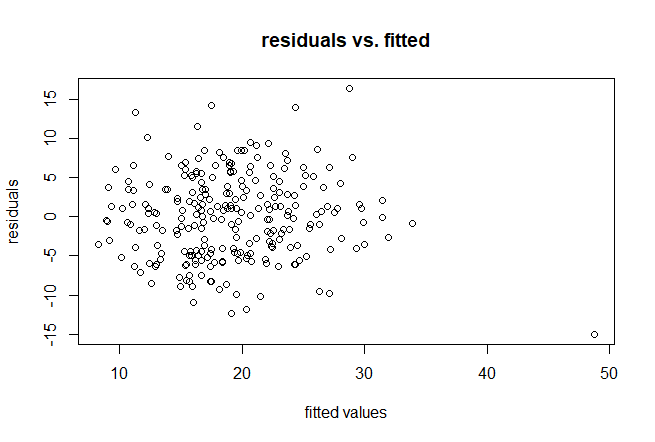
\includegraphics[width=8cm,height=1cm]{1.png}
\end{figure}\\
Next one is the same.
\begin{figure}[ht]
    \centering
	\includegraphics[width=8.5cm,height=2.7cm]{4.png}
\end{figure}
\subsection{Speed}
To speed up our codes, we try to simplify the algorithm and avoid using too many loops. Actually we do meet many situations and we have to deal with it but slow the code at the same time.\newpage 
\begin{flushleft}
We run the test codes and get the result.
\end{flushleft}
\begin{figure}[ht]
    \centering
	\includegraphics[width=3.5cm,height=1cm]{5.png}
\end{figure}
\subsection{Scalability}
It works well for scalability and it almost shows linear relationship between time and data scale.
\begin{figure}[ht]
    \centering
	\includegraphics[width=8cm,height=5cm]{6.png}
\end{figure}
\section{Extra Data Test}
Additionally, to show the ability of the algorithm, we create our own data to deeply test our algorithm.
First we create 60s data to test, then print the left figure: The blue line means our prediction and the red line shows the true value. Our prediction is 5 seconds earlier than the real one.\\
\begin{figure}[ht]
	\centering
	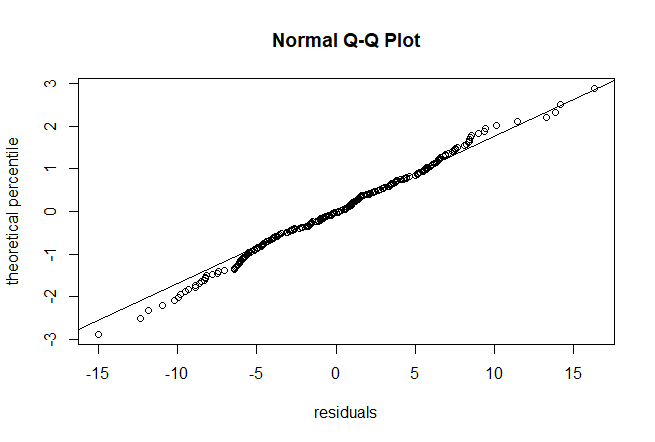
\includegraphics[width=8cm,height=6cm]{2.png}
	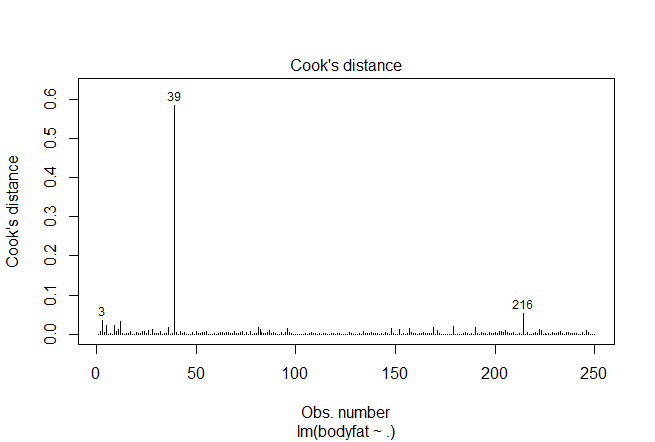
\includegraphics[width=8cm,height=6cm]{3.png}  
\end{figure}
\newline
There is another special case on the right which has a break points. Our algorithm overcome the problem which the professor meet with and deal with it properly in the future.\\
\newline
Actually, \textbf{if the slope varies significantly in y\_t, the algorithm may perform poorly.} That's why we need to improve our algorithm.
\end{document}